\chapter{Klassendiagramme - erweiterte Konzepte und Paketdiagramme}


\section{Lernziele}

\begin{itemize}
    \item für kleinere Projekte qualitätssichernde Maßnahmen planen und verfolgen können
    \item Tests planen und dokumentieren können
    \item gefundene Fehler geeignet verwalten können
\end{itemize}

\newpage

\section{Darstellung der erweiterten Konzepte}\label{sec:darstellung-der-erweiterten-konzepte}

\textbf{Erweiterte Konzepte} werden vor allem im \textbf{Detailentwurf} verwendet.\\

\noindent
Dabei werden \textit{nicht} alle Konzepte durch eigene \textbf{Symbolik} dargestellt: Mitunter werden gleiche Symbole mit unterschiedlichen \textbf{Keywords} (\textit{Schlüsselwörter}) versehen.\\

\noindent
Keywords werden in französischen Anführungszeichen (\textit{guillemets}: \guillemotleft Keyword\guillemotright) geschrieben und sind durch die Spezifikation vorgegeben (s.~\cite[746 ff.]{OMG17}).

\noindent
Durch Keywords werden auch \textbf{Standardstereotypen} ausgewiesen.\\
\textbf{Stereotypen} sind Erweiterungen von vorhandenen Modellierungkonzepten auf der Ebene des UML Metamodells und spezifizieren diese näher für einen vorgesehen Verwendungszeck.\\

\noindent
Stereotypen, die einer Anwendungsdomäne zugeordnet werden können, können in \textbf{Profile}s zusammengefasst werden\footnote{
Darstellung etwa: Package-Symbol mit Schlüsselwort \guillemotleft profile\guillemotright. Die UML definiert bspw. das \textit{UML Testing Profile}: \url{https://www.omg.org/spec/UTP2/}, abgerufen 05.05.2024
}


\section{Begriffe und Elemente in Klassendiagrammen}

\subsection{Komposition}
Bei einer \textbf{Komposition} handelt es sich um eine \textit{Ganzes}-\textit{Teile}-Beziehung, bei der das \textit{Ganze} verantwortlich für die Erstellung und Beseitigung der \textit{Teile} ist.
Außerdem sind die \textit{Teile} an die \textbf{Existenz} des \textit{Ganzen} gebunden.\\
\textit{Teile} gehören immer zu \textit{genau einem} \textit{Ganzen}.\\
Eine Komposition wird dargestellt durch eine gefüllte Raute an der Klassenbox, die das \textit{Ganze} repräsentiert.\\

\noindent
Um sicherzustellen, dass ein Teil immer nur zu einem \textit{Ganzen} gehört, kann bspw. in einer Methode, die Informationen über ein Teil zurückliefert, eine Kopie des Teils zurückgegeben werden.
Dadurch ist sichergestellt, dass die Referenz auf ein existierendes Objekt nicht mehrfach verwendet werden kann.

\subsection{Aggregation}
Eine \textbf{Aggregation} ist in ihrer \semantischen Aussage unscharf (vgl.~\cite[40]{Buh09}).\\
Auch hier geht es um eine \textit{Ganzes}-\textit{Teile}-Beziehung, aber die \textit{Teile} können zu mehreren verschiedenen \textit{Ganzen} gehören.
Außerdem kann ein Teil dem \textit{Ganzen} jederzeit wieder entnommen werden und das \textit{Ganze} ist nicht verantwortlich für das Erstellen der \textit{Teile}, weshalb Implementierungen beim Hinzufügen von Teilen oft schon fertige Objekte erwarten, die jeweils eines der \textit{Teile} repräsentieren.

\subsection{Schnittstellen}
\textbf{Schnittstellen} geben eine Vertrag vor, den implementierende Klassen erfüllen:

\begin{itemize}
    \item eine Klasse, die die Schnittstelle implementiert, muss die deklarierten Operationen umsetzen
    \item eine einzelne Klasse kann beliebig viele Schnittstellen implementieren
    \item eine einzelne Schnittstelle kann von beliebig vielen Klassen implementiert werden
    \item Schnittstellen können andere Schnittstellen generalisieren
\end{itemize}

\noindent
Schnittstellen können mit dem Stereotyp \textcolor{blue}{\guillemotleft interface\guillemotright} über ihrem Namen in der Klassenbox gekennzeichnet werden.

\subsection{Abstrakte Klassen}
\textbf{Abstrakte Klassen} werden mit \code{{abstract}} gekennzeichnet\footnote{
``after or below its name`` (\cite[101]{OMG17})
}, oder der Klassenname wird \textit{kursiv} gesetzt.\\
Abstrakte Klassen können nicht instanziiert werden und können abstrakte Methoden und Methoden mit Implementierungen enthalten.\\
Hat eine Klasse eine abstrakte Methode, ist diese automatisch abstrakt.\\
Wird eine abstrakte Klasse abgeleitet, und die ableitende Klasse ist nicht abstrakt, müssen die abstrakten Methoden in der ableitenden Klasse implementiert werden.

\subsection{Assoziationsklasse (Attributierte Assoziation)}
Eine \textbf{Assoziationsklasse} erlaubt das Hinzufügen von Operationen und Attributen zu einer Assoziation (\cite[43]{Buh09}).

\blockquote[{\cite[277]{Oes05}}]{
Eine attributierte Assoziation ist immer dann nahe liegend, wenn Attribute oder Operationen gefunden werden, die weder der einen noch der anderen Klasse zugeordnet werden können, weil sie nämlich Eigenschaften der Beziehung selbst sind.
}.

\begin{tcolorbox}
Bei einer attributierten Assoziation dürfen zwei beteiligte Objekte maximal nur eine Beziehung zueinander haben (vgl.~\cite[277]{Oes05})\footnote{
\textit{Ostereich} führt dies ebenda auf Seite 278 weiter aus, in dem er beschreibt, wie eine attributierte Assoziation für ein \textit{Beschäftigtenverhältnis} zwischen \textit{Mitarbeiter} und \textit{Unternehmen} modelliert wird. Dabei wird davon ausgegangen, dass ein \textit{Mitarbeiter} nur über \textit{ein} Arbeitsverhältnis mit einem \textit{Unternehmen} in Beziehung stehen kann. Bestehen mehrere Arbeitsverhältnisse (\textit{Mitarbeiter} hat zu unterschiedlichen Zeitpunkten für das \textit{Unternehmen} gearbeitet), kann die attributierte Assoziation nicht verwendet werden.
}.
\end{tcolorbox}

\noindent
Wird eine attributierte Assoziation in eine gewöhnliche Assoziation transformiert, muss darauf geachtet werden, die Multiplizitäten richtig zu setzen (s. Abbildung~\ref{fig:assoziationsklasse}).

\begin{figure}
    \centering
    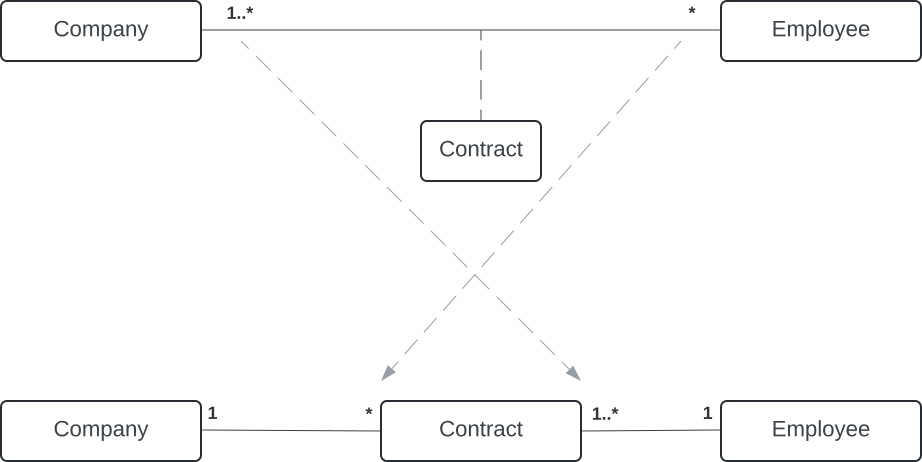
\includegraphics[scale=0.4]{part three/Klassendiagramme - Erweiterte Konzepte und Paketdiagramme/img/assoziationsklasse}
    \caption{Darstellung einer Assoziation mit Hilfe einer Assoziationsklasse (oben) sowie Transformation in gewöhnliche Assoziationen (unten). (Quelle: in Anlehnung an \cite[279, Abb. 4.4-11]{Oes05})}
    \label{fig:assoziationsklasse}
\end{figure}

\subsection{Templates (generische / parametrisierbare Klassen)}
Klassen, die als \textbf{Template} gekennzeichnet sind, stellen ``eine Beschreibung einer Klasse mit einem oder mehreren formalen Parametern`` (\cite[253]{Bal05})\footnote{
s.a. \cite[103 ff.]{OMG17}
} dar.\\

\noindent
Hierüber lassen sich bspw. Java-\texbf{Generics} modellieren.\\

\noindent
Eine Klasse wird zunächst mit einem Parameternamen gekennzeichnet.
Für einen konkreten Anwendungsfall wird dann eine Klasse als konkreter Parametertyp gebunden (s. Abbildung~\ref{fig:template} und nachfolgender Quelltext, beides nach \cite[81 f.]{Fow03b}).

\begin{minted}[mathescape,
    linenos,
    numbersep=5pt,
    gobble=2,
    fontsize=\small]{java}
    class RainbowBucket <T extends ValuableElement>{
    }

    RainbowBucket<Gold> potOfGolf;

\end{minted}
\begin{figure}
    \centering
    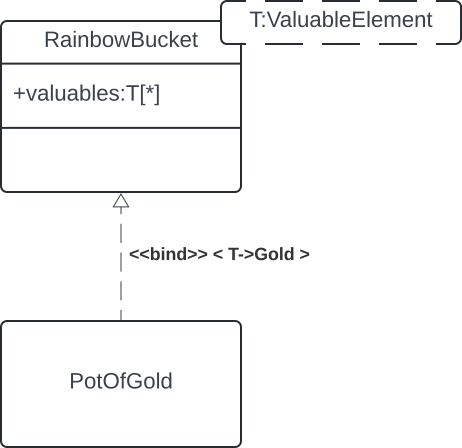
\includegraphics[scale=0.4]{part three/Klassendiagramme - Erweiterte Konzepte und Paketdiagramme/img/template}
    \caption{Parametrisierbare Klasse RainbowBucket. (Quelle: eigene)}
    \label{fig:template}
\end{figure}

\blockquote[{\cite[82, Hervorhebungen i.O.]{Fow03b}}]{
Using a derivation [Anm.: die Verwendung einer parametrisierbaren Klasse wie in Abbildung~\ref{fig:template} gezeigt] is \textit{not}
the same as subtyping, however. You are not allowed to add features to the bound element, which is completely specified by its template; you are adding only restricting type information. If you want to create features, you must create a subtype.
}
\section{Einsatzbereich von Paketdiagrammen}

\textbf{Paketdiagramme} zeigen Pakete und ihre Abhängigkeiten und werden in frühen Designphasen genutzt, um Strukturen (großer Systeme) aufzuzeigen.\\
Durch die Gruppierung können Details weggelassen werden.\\

\noindent
Eine Abhängigkeit zwischen zwei Paketen gibt die Abhängigkeit darin enthaltener Elemente wieder.\\

\noindent
Ein Paket gruppiert Elemente und definiert Namensräume für die darin enthaltenen Elemente.\\

\noindent
Paketdiagramme können auch dazu genutzt werden, um UML Modelle zu vereinfachen: Logisch zusammengehörende UML Elemente werden in ein Paket gelegt.\\

\noindent
Folgende Symbolik kann verwendet werden, um Pakete in Diagrammen zu zeigen:

\begin{itemize}
    \item \textbf{Paketsymbol}
    \item \textbf{Fully Qualified Name}\footnote{
    s. \url{https://en.wikipedia.org/wiki/Fully_qualified_name}, abgerufen 06.05.2024
    }
    \item \textbf{Symbole in Kombination mit Namen}
\end{itemize}

\noindent
Es können immer nur \textbf{public} Elemente in anderen Paketen gesehen werden.
\textit{Buhl} weist darauf hin, dass dies erlaubt, ``Pakete mit Fassaden auszustatten. Das bedeutet, es gibt nur eine public Klasse (Facade) und alle anderen Klassen sind privat.`` (\cite[46]{Buh09}).\\

\begin{tcolorbox}
    Elemente sollten so in Paketen gruppiert werden, dass ihr \textbf{funktionaler Zusammenhalt} (\textit{Kohäsion}, s. Abschnitt~\ref{subsec:hohe-kohasion}) klar wird\\.
    Hierdurch kann vermieden werden, dass Änderungen einer Klasse eines Paketes auch Änderungen außerhalb des Paketes erfordern.\\
    Außerdem erhöht sich die Wahrscheinlichkeit, dass einzelne Pakete als solche in anderen Projekten wiederverwendet werden können.
\end{tcolorbox}

\section{Begriffe und Elemente in Paketdiagrammen}

Beziehungen zwischen Paketen können über folgende Schlüsselwörter deutlich gemacht werden:

\subsection{\guillemotleft import\guillemotright}
Beschreibt einen \textbf{public-Import} zwischen Quell- und Zielpaket.
Erlaubt dem Quellpaket eine Verwendung der öffentlichen Elemente des Zielpaketes unter Verwendung des unqualifizierten und des qualifizierten Namens.\\
Die importierten Elemente sind auch für Pakete sichtbar, die das Quellpaket importieren.
So findet in Abbildung~\ref{fig:import-access} ein Import von \code{P1} in \code{P3} statt. \code{P4} importiert wiederum \code{P3} und kann auch direkt auf die Klassen \code{P1::A}, \code{P1::B} und \code{P3::B} zugreifen.\\

\subsection{\guillemotleft access\guillemotright}
Beschreibt einen \textbf{privaten Import} zwischen Quell- und Zielpaket.
In Abbildung~\ref{fig:import-access} findet ein privater Import von \code{P2} in \code{P3} statt.
In \code{P3} kann folglich ohne qualifizierenden Namen auf \code{P2::C} und \code{P2::D} zugegriffen werden, nicht jedoch von \code{P4} aus.\\
Der Import eines Paketes in \textbf{Java} entspricht der \guillemotleft access\guillemotright-beziehung

\blockquote[{\cite[307, Hervorhebung i.O.]{Bal05}}]{
Wenn ein \textbf{Paket-Import} [Anm.: import/access] spezifiziert ist, dann können die Elemente des importierten Pakets im importierenden Paket ohne qualifizierenden Namen verwendet werden.
}

\begin{figure}
    \centering
    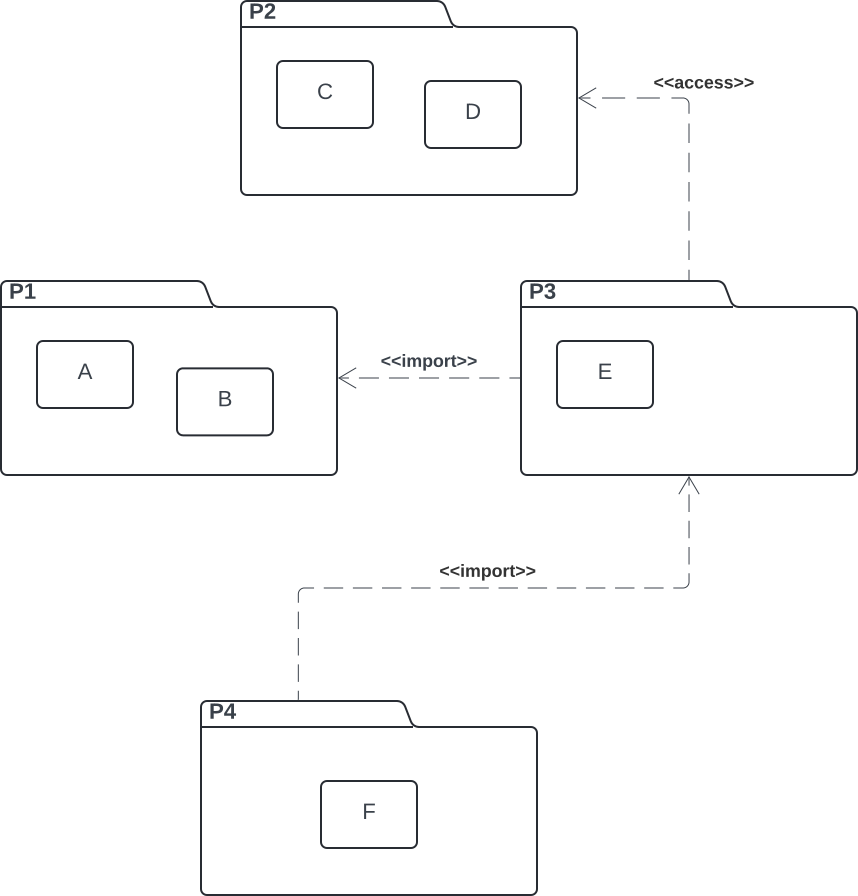
\includegraphics[scale=0.4]{part three/Klassendiagramme - Erweiterte Konzepte und Paketdiagramme/img/import-access}
    \caption{Verwendung von \guillemotleft import\guillemotright / \guillemotleft access\guillemotright in Paketdiagrammen. (Quelle: in Anlehnung an~\cite[308, Abb. 6.8-3]{Bal05})}
    \label{fig:import-access}
\end{figure}

\subsection{\guillemotleft merge\guillemotright}
Bei einem \textbf{merge} werden Elemente eines Zielpaketes in das Quellpaket kopiert und können dann verändert werden (vgl.~\cite[307]{Bal05}).\\
Durch einen Merge können Elemente gleichen Namens gemischt werden.
Abbildung~\ref{fig:import-merge} verdeutlicht dies: Das Zielpaket \code{Z} wird in Quellpaket \code{Q} \textit{gemergt}.
Unabhängig davon, ob \code{Q} bereits eine Klasse \code{A} oder \code{B} enthält, wird in \code{Q} jeweils eine Oberklasse \code{Z::A} bzw. \code{Z::B} eingefügt.
Existiert in \code{Q} keine Klasse \code{A} oder \code{B}, wird diese entsprechend eingefügt (vgl. \textit{einfacher Paket-Merge}, \cite[308]{Bal05}).


\begin{figure}
    \centering
    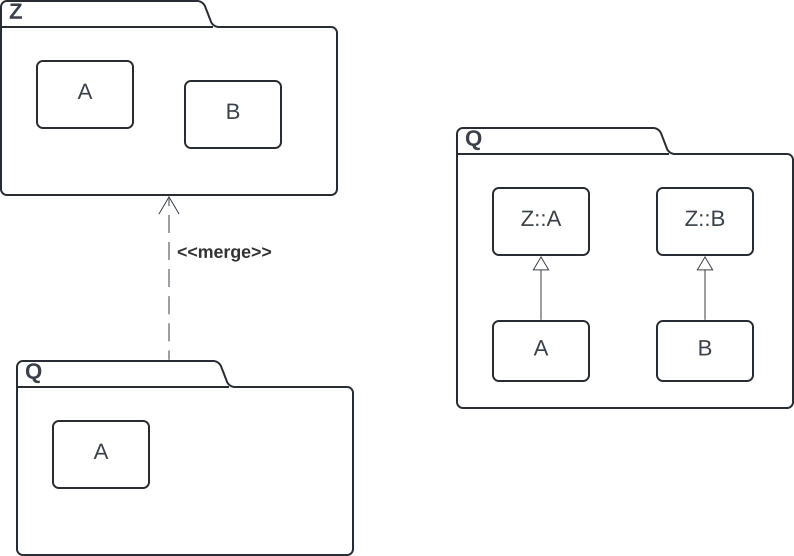
\includegraphics[scale=0.4]{part three/Klassendiagramme - Erweiterte Konzepte und Paketdiagramme/img/import-merge}
    \caption{Einfacher Paket-Merge. (Quelle: in Anlehnung an~\cite[308, Abb. 6.8-4]{Bal05})}
    \label{fig:import-merge}
\end{figure}

\newpage
\section{Zusammenfassung}

\begin{itemize}
    \item Anforderungen lassen sich bei Projekten vorab nicht genügend festlegen.
    \item Fehlt im Team die Erfahrung oder werden neue Technologien eingesetzt, ist ein ausgereifter Entwurf nicht machbar.
    \item Bei großen Projekten würde man unter diesen Voraussetzungen mit dem Wasserfallmodell nicht flexibel genug sein,
    um auf Änderungen reagieren zu können.
    \item Aus diesem Grund gibt es alternative Modelle, die eingesetzt werden können:
        \begin{itemize}
            \item \textbf{inkrementell}: Aufteilung der Anforderungen, so dass Teilsysteme umgesetzt und an den Kunden ausgeliefert werden können
            Die Teilsysteme werden sequentiell bearbeitet.
            \item \textbf{iterativ}: In Iterationen wird das Projekt in Zeitabschnitte unterteilt, in denen die Anforderungen umgesetzt werden; entsprechend dem Spiralmodell zunächst die risikoreichsten.
            Vorhergehende Ergebnisse werden in darauffolgenden Iterationen weiterbearbeitet.
            Ein bekanntes iteratives Modell ist \textit{RUP}, bei dem einzelne Phasen Ergebnis-Artefakte liefern, wie Anwendungsfälle oder Klassendiagramme.
            \item \textbf{nebenläufig}: Die Aufgaben werden aufgeteilt in parallel (oder nacheinander) bearbeitbare Aufgaben, die dann von den Mitarbeitern umgesetzt werden.
        \end{itemize}
    \item Die genannten Modelle werden häufig nicht isoliert betrachtet, sondern je nach Projekt auch kombiniert, insb. bei dem \textbf{agilen Vorgehen}.
\end{itemize}

\newpage


